\documentclass[a4paper,11pt]{article}
\usepackage{amsmath}
\usepackage{amsthm}
\usepackage{amssymb}
\usepackage{algorithm}
\usepackage{algorithmic}
\usepackage{polski}
\usepackage[utf8]{inputenc}
\usepackage{tikz}

\theoremstyle{definition}
\newtheorem{definition}{Definition}[section]
\newtheorem{theorem}{Theorem}[section]
\newtheorem{lemma}{Lemma}[section]
\newtheorem{corollary}{Corollary}[lemma]

\title{String-matching on ordered alphabets \\ \large W oparciu o ,,String-matching on ordered alphabets"\\ Maxime Crochemore}
\author{Jan Mełech}
\date{}

\begin{document}

\maketitle

\section{Notacja}
\begin{itemize}
    \item $p(t)$ - najmniejszy okres słowa $t$
    \item $p'(t)$ - okres słowa $t$ odpowiadający największemu silnemu prefikso-sufiksowi
\end{itemize}

\section{Wstęp}

Autor przedstawia liniowy algorytm do znajdowania wzorca w tekście. Przedstawiony algorytm należy do ogólniejszej klasy algorytmów skanujących tekst od lewej do prawej i wykonujących odpowiednie przesunięcia. Zaproponowany algorytm jest pierwszym algorytmem z tej klasy, który wymaga stałej ilości pamięci.


\section{Główna idea algorytmu}

Przyjmijmy, że mamy sytuację jak na rysunku \ref{fig:mismatch}. Oznaczmy $y$ - prefiks wzorca już dopasowanego, $b$ - pierwszy znak w tekście, który jest różny od odpowiadającego mu znaku we wzorcu (lub kolejny znak w tekście gdy znaleźliśmy dopasowanie).
\par 
Algorytmy MP I KMP wykonują w takiej sytuacji przesunięcia odpowiednio o $p(y)$ i $p'(y)$, jednak oba podejścia wymagają pamięci wielkości proporcjonalnej do wielkości wzorca. 
\par 
Crochemore stosuje nieco inne podejście. Najpierw zauważa, że najlepszym możliwym przesunięciem jest $p(yb)$. Następnie na podstawie dekompozycji słowa $yb$ opartej na maksymalnym sufiksie oblicza przybliżoną wartość  $p(yb)$. Samo obliczenie będzie wymagało stałej liczby komórek pamięci, zaś przybliżenie będzie wystarczająco dobre, aby osiągnąć liniową złożoność czasową.

\begin{figure}
    \centering
    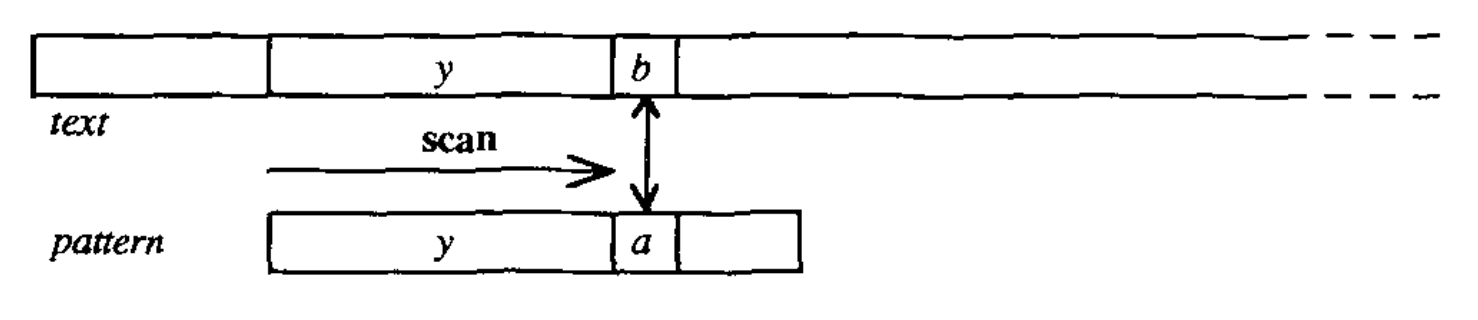
\includegraphics[scale=0.3]{mismatch.PNG} \\
    \caption{Niedopasowanie tekstu ze wzorcem}
    \label{fig:mismatch}
\end{figure}

\section{Okresy słowa, a maksymalne sufiksy}
Niech $v$ będzie maksymalnym leksykograficznie sufiksem niepustego słowa $x$. Przedstawmy $v$ jako $w^ew'$, gdzie $e \geq 1$, $|w| = p(v)$, zaś $w'$ jest właściwym prefiksem $w$. Niech $u$ będzie prefiksem $x$, takim że $x = uv = uw^ew'$. Czwórkę $(u, w, e, w')$ będziemy nazywać MS-dekompozycją (skrót z angielskiego \textit{maximum-suffix decomposition}) słowa $x$.
\par
Na początku przywołajmy lemat, że element $w$ w MS-dekompozycji nie może mieć właściwego prefikso-sufiksu:
\begin{lemma}\label{lem:w_is_borderless}
Niech $uw^ew'$ będzie MS-dekompozycją niepustego słowa $x$. Wtedy zachodzi $p(w) = |w|$.
\end{lemma}
\par
Następnie pokażemy w jaki sposób możemy oszacować najmniejszy okres słowa za pomocą jego MS-dekompozycji:
\begin{lemma}\label{lem:maximul_suffix_properties}
Niech $uw^ew'$ będzie MS-dekompozycją niepustego słowa $x$. Wtedy zachodzą następujące własności:
\begin{enumerate}
    \item jeśli $u$ jest sufiksem $w$, to $p(x) = p(v)$,
    \item $p(x) > |u|$,
    \item jeśli $|u| \geq |w|$, to $p(x) > |v| = |x| - |u|$,
    \item jeśli $u$ nie jest sufiksem $w$ oraz $|u| < |w|$, to $p(x) > min(|v|, |uw^e|)$.
\end{enumerate}
\begin{proof}


\begin{enumerate}
    \item Gdy $u$ jest sufiksem $w$, nietrudno zauważyć, że $|w|$ jest najmniejszym okresem $x$. Zatem $p(x) = |w| = p(v)$.
    \item Gdyby $p(x) \leq |u|$, to w $x$ istniałoby drugie wystąpienie $v$ w $x$ niebędące sufiksem $x$. Zatem $x$ moglibyśmy zapisać jako $u'vv'$, gdzie $|u'| < |u|$ oraz $|v'| > 0$. Z drugiej strony, $vv' > v$ co stoi w sprzeczności, że $v$ jest maksymalnym sufiksem $x$.   
    \item Załóżmy przeciwnie, że $p(x) \leq |v|$. Zatem w $x$ można znaleźć drugie wystąpienie $u$ w $x$ niebędące prefiksem $x$, które przecina $v$. Skoro $|u| \geq |w|$, to istnieje $z$ sufiks $u$, który jest jednocześnie prefiksem $w$, jak pokazane na rysunku \ref{fig:u_suffix_is_prefix_w}. Teraz możemy zapisać $v = zz'$. Skoro $v$ jest maksymalnym sufiksem to dostajemy $zv < v = zz'$. Z tego wnioskujemy, że $v < z'$, sprzeczność z maksymalnością $v$.
    \begin{figure}
    \centering
    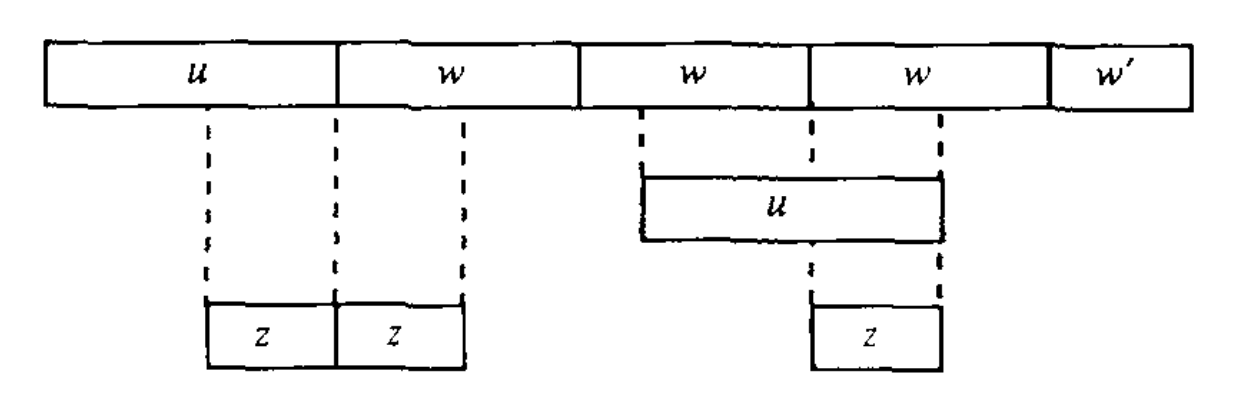
\includegraphics[scale=0.3]{u_suffix_is_prefix_w.PNG} \\
    \caption{Sufiks $u$ jako prefiks $w$}
    \label{fig:u_suffix_is_prefix_w}
    \end{figure}
    \item Załóżmy przeciwnie, że $p(x) \leq min(|v|, |uw^e|)$. Z $p(x) \leq |v|$ wynika, że istnieje drugie wystąpienie $u$ w $x$ niebędące prefiksem $x$. Natomiast z $p(x) \leq |uw^e|$ możemy wysnuć wniosek, że to drugie wystąpienie musi się przecinać z $w^e$. Jeżeli przecinałoby się z granicą dwóch kolejnych słów $w$ w $w^e$ lub z granicą pomiędzy ostatnim $w$ i $w'$ to z poprzedniego podpunktu otrzymujemy sprzeczność. Zatem $u$ musi być podsłowem $w$ różnym od jego sufiksu (z założenia). Z okresowości po $u$ musi nastąpić $w$, co implikuje sytuację widoczną na \ref{fig:w_is_border_w}, w której dostajemy, że $w$ ma właściwy prefikso-sufiks, co daje nam sprzeczność z lematem \ref{lem:w_is_borderless}
    \begin{figure}
    \centering
    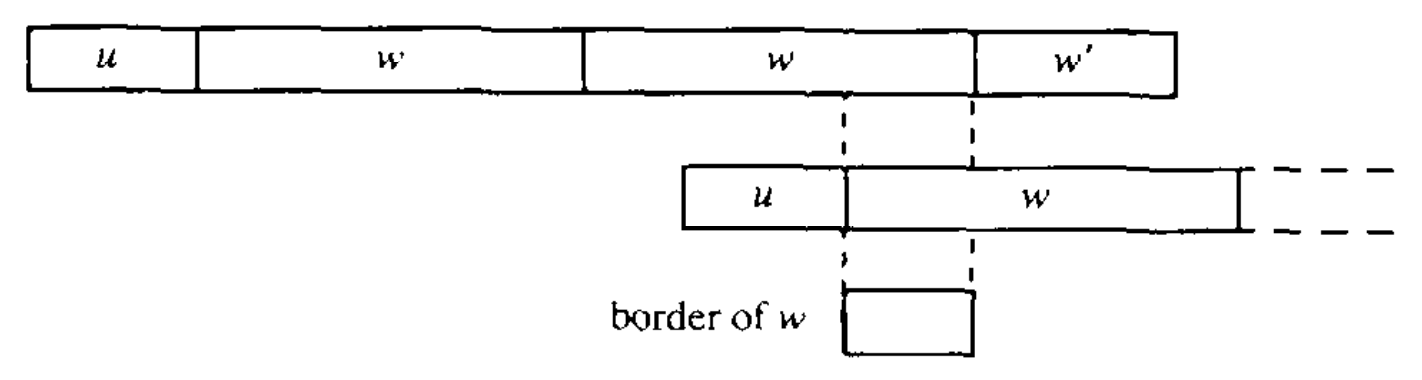
\includegraphics[scale=0.3]{w_is_border_free.PNG} \\
    \caption{$w$ nie może mieć właściwego prefikso-sufiksu}
    \label{fig:w_is_border_w}
    \end{figure}
\end{enumerate}
\end{proof}
\end{lemma}

\begin{corollary}\label{col:MS_decomposition_bounds}
Niech $uw^ew'$ będzie MS-dekompozycją niepustego słowa $x$. Jeżeli $u$ jest sufiksem $w$, to $p(x) = p(x) = |w|$. W przeciwnym przypadku, $p(x) > max(|u|, min(|v|, |uw^e|)) \geq |x|/2$.

\end{corollary}

\begin{proof}
Jeżeli $u$ jest sufiksem $w$ to na podstawie pierwszego podpunktu lematu \ref{lem:maximul_suffix_properties} dostajemy $p(x) = p(x) = |w|$. W przeciwnym przypadku, na podstawie pozostałych podpunktów lematu \ref{lem:maximul_suffix_properties} otrzymujemy nierówność $p(x) > max(|u|, min(|v|, |uw^e|))$. Jeżeli $|u| \geq |x|/2$ to od razu dostajemy tezę. Z drugiej strony, jeżeli $|u| < |x|/2$, to $|v| \geq |x|/ 2$. Dodatkowo, $|uw^e| = |x| - |w'| > |x| / 2$, ponieważ $2 |w'| < |w'| + |w| \leq |v| < |x|$.
\end{proof}

\section{Obliczanie MS-dekompozycji}
MS-dekompozycję słowa $x$ będziemy przechowywać za pomocą MS-czwórki $(i,j,k,p)$. MS-czwórka $(i,j,k,p)$ to cztery liczby charakteryzujące w pełni MS-dekompozycję $x$: 

\[ i = |u|, j = |uw^e|, k = |w'|+1, p = |w| = p(v) \]
gdzie $x = uw^ew'$.

\subsection{Optymalizowanie obliczania MS-dekompozycji}
Gdyby obliczać w każdej iteracji MS-dekompozycję słowa $yb$ to dla pary $t = a^n, w = a^m, n > m$ nasz algorytm zajmowałby $O(|t||w|)$ czasu. Rozwiązaniem tego problemu jest wykorzystywanie MS-dekompozycji obliczonych w poprzednich iteracjach pod pewnymi warunkami zawartymi w następującym lemacie:
\begin{lemma}\label{lem:maximul_suffix_of_prefix}
Niech $(u, w, e, w')$ będzie MS-dekompozycją niepustego słowa $x = uw^ew'$. Załóżmy, że $p(x) = |w|$. Wtedy, jeżeli $e > 1$, to $(u, w, e-1, w')$ jest MS-dekompozycją słowa $x' = uw^{e-1}w'$.
\end{lemma}


\subsection{Pseudokod}

Do obliczania MS-dekompozycji będziemy używać pomocniczej metody next\_maximal\_suffix. Na wejściu mamy słowo $w$ długości $m$ or MS-czwórkę $(i,j,k,p)$ dla pewnego słowa $z$ będącego prefiksem $w$. Sama metoda polega na iterowaniu się po całym słowie $w$ zaczynając od prefiksu $z$ i odpowiednim aktualizowaniu poszczególnych wartości MS-czwórki w zależności od tego czy znaleźliśmy nowy maksymalny sufiks czy nie.

\begin{algorithm}[H]
\caption{next\_maximal\_suffix$(w[1] \ldots w[m], (i, j, k, p))$}\label{alg:next_maximal_suffix}
\begin{algorithmic} 
\STATE $t\_pos \gets 0,  w\_pos \gets 1$
\STATE $(i,j,k,p) \gets (0,1,1,1)$
\WHILE {$j + k \leq m$}
    \IF {$w[i + k] = w[j + k]$}
        \IF {$k = p$}
            \STATE $j \gets j + p, k \gets 1$
        \ELSE
            \STATE $k \gets k + 1$
        \ENDIF
    \ELSIF {$w[i + k] > w[j + k]$}
        \STATE $j \gets j + k, k \gets 1, p \gets j - i$
    \ELSE
        \STATE $i \gets j, j \gets i + 1, k \gets 1, p \gets 1$
    \ENDIF
\ENDWHILE
\RETURN $(i, j, k, p)$

\end{algorithmic}
\end{algorithm}

\section{Główny algorytm}
Przedstawmy główny algorytm string\_matching. Wpisuje się on w klasyczny schemat algorytmów skanujących tekst od lewej do prawej i wykonujących przesunięcia. Omówmy najważniejszą część tego algorytmu, czyli obliczenie przesunięcia. Przyjmijmy oznaczenia z rysunku \ref{fig:mismatch}. Najpierw obliczamy MS-czwórkę słowa $yb$ używając metody next\_maximal\_suffix, dostając $yb = uw^ew'$. Następnie na bazie wniosku \ref{col:MS_decomposition_bounds} sprawdzamy czy $u$ jest sufiksem słowa $w$:
\begin{itemize}
    \item jeżeli tak, to $p(yb) = |w|$ i o tyle możemy przesunąć tekst. Dodatkowo sprawdzamy czy $j - i > p$ (co jest równoważne sprawdzeniu $e > 1$) , aby w miarę możliwości nie obliczać następnej MS-czwórki od początku (na podstawie lematu \ref{lem:maximul_suffix_of_prefix}). 
    \item jeżeli nie, to przesuwamy o $max(|u|, min(|v|, |uw^e|))$.
\end{itemize}

\subsection{Dowód poprawności}
W obu przypadkach wartość przesunięcia nie przekracza $p(yb)$ zatem nic nie przeoczymy na przesunięciach, a na sprawdzanych pozycjach w oczywisty sposób poprawnie zwrócimy wystąpienia wzorca.

\subsection{Skrót dowodu złożoności}
Najpierw zauważmy, że podczas sprawdzania czy $u$ jest sufiksem $w$ porównamy co najwyżej $i = |u|$ znaków z tekstu $t[t\_pos + 1] \ldots t[t\_pos + i]$. W każdej iteracji tekst przesuniemy o co najmniej $i$, zatem porównań znaków wykonanych w linii 14 będzie co najwyżej $|t|$ podczas całego algorytmu. 

Nastęnie autor pokazuje, że każde pozostałe porównanie w algorytmie string\_matching zwiększy wartość wyrażenia $5 \cdot t\_pos + w\_pos + i + j + k$. Na końcu wyrażenie osiągnie wartość $5|t| + 8$, co da nam liniową złożoność czasową.

Możemy prześledzić jak zachowuje się wyrażenie $5 \cdot t\_pos + w\_pos + i + j + k$:
\begin{itemize}
    \item można zauwazyć, że każde porównanie znaków w metodzie next\_maximal\_suffix zwiększa wartość wyrażenia $i + j + k$ o co najmniej 1,
    \item pomyślne porównanie znaków w trakcie skanu zwiększa $w\_pos$ o 1,
    \item niepomyślne porównanie znaków rozkłada się na 3 przypadki, każdy z nich jest dość techniczny - pozwoliłem je sobie pominąć.
\end{itemize}

\begin{algorithm}[H]
\caption{string\_matching$(t, w, n, m)$}
\begin{algorithmic}[1]
\STATE $t\_pos \gets 0,  w\_pos \gets 1$
\STATE $(i,j,k,p) \gets (0,1,1,1)$
\WHILE {$t\_pos \leq n - m$}
    \WHILE {$ w\_pos \leq m$ \AND $t[t\_pos +  w\_pos] = w[ w\_pos]$}
        \STATE $ w\_pos \gets  w\_pos + 1$
    \ENDWHILE
    
    \IF {$ w\_pos = m + 1$}
        \RETURN $t\_pos + 1$
    \ENDIF
    
    \IF {$t\_pos = n - m$}
        \STATE break
    \ENDIF
    
    \STATE $(i,j,k,p) \gets next\_maximal\_suffix(w[1] \ldots [ w\_pos-1]t[t\_pos +  w\_pos], (i, j, k, p))$
    \IF {$w[1] \ldots w[i]$ is suffix of prefix of length $p$ of $w[i+1] \ldots [ w\_pos-1]t[t\_pos +  w\_pos]$}
        \STATE $t\_pos \gets t\_pos + p$, $ w\_pos \gets  w\_pos - p + 1$
        \IF {$j - i > p$}
            \STATE $j \gets j - p$
        \ELSE
            \STATE $(i,j,k,p) \gets (0,1,1,1)$
        \ENDIF
    \ELSE
        \STATE $t\_pos \gets t\_pos + max(i, min( w\_pos - i, j)) + 1$, $ w\_pos \gets 1$
        \STATE $(i,j,k,p) \gets (0,1,1,1)$
    \ENDIF
\ENDWHILE

\end{algorithmic}
\end{algorithm}


\end{document}